\documentclass[9pt]{beamer}

\geometry{paperwidth=213.3mm,paperheight=120mm}

\usetheme[{titleformat plain}=smallcaps,
           titleformat title=smallcaps,
           titleformat subtitle=regular,
           titleformat section=smallcaps,
           titleformat frame=smallcaps,
           % numbering=fraction,
          ]{metropolis}
% \usepackage{appendixnumberbeamer}

\definecolor{mLightGreen}{HTML}{14B03D}
\definecolor{vpGreen}{HTML}{66c2a5}
\definecolor{vpOrange}{HTML}{fc8d62}
\providecommand{\iRef}[1]{{\color{mLightGreen}\small $[$#1$]$}}

\usepackage{../_style/common}
\usepackage{../_style/defs}

\usepackage{alphalph}

\usepackage{enumitem}
\setenumerate[1]{%
      label=\protect\usebeamerfont{enumerate item}%
      \protect\usebeamercolor[fg]{enumerate item}%
      \insertenumlabel.}
\setitemize{label=\usebeamerfont*{itemize item}%
    \usebeamercolor[fg]{itemize item}
      \usebeamertemplate{itemize item}}

\graphicspath{{pictures/}{../_pictures/}{../2022-Gargnano/pictures/}}

\usepackage[symbol]{footmisc}
\renewcommand{\thefootnote}{\fnsymbol{footnote}}

\title{Parton Distribution Functions}
\subtitle{
    \textit{solving the probabilistic inverse problem} - or
    \textit{\enquote{How to learn a function}}
}
\date{August, 2022}
\author{Alessandro Candido}
%\institute{N3PDF}
\titlegraphic{
    \raisebox{10pt}[0pt][0pt]{
\includegraphics[width=2.5cm]{../_logos/nnpdf_logo.pdf}}\hspace*{10pt}
    \hfill
    \raisebox{5pt}[0pt][0pt]{
\includegraphics[height=0.8cm]{../_logos/n3pdf_logo.pdf}}\hspace*{10pt}
    
\includegraphics[height=1.3cm]{../_logos/erc_logo1.png}

    \vfill\vspace*{230pt}
    
\includegraphics[height=1cm]{../_logos/unimi_logo.png}\hfill
    
\includegraphics[height=1cm]{../_logos/infn_logo.png}\\
    \vspace*{5pt}
    {
        \fontsize{3pt}{3.5pt}\selectfont
        \begin{center}
            This project has received funding from the European Union's Horizon
            2020 research and innovation programme under grant agreement No
            740006\quad 
\includegraphics[height=5pt]{../_logos/eu-flag.jpg}
        \end{center}
    }
}

\begin{document}

\maketitle

\setlist[description]{font=\quad\normalfont\bfseries\scshape\space}
\metroset{block=fill}

\section{The Physics}

\begin{frame}{Theoretical Picture of a Collision}
    \begin{columns}
        \begin{column}{0.5\textwidth}
            In order to describe a \textit{\textbf{collision}} a lot of ingredients are
            involved:
            \begin{itemize}
                \item a \textbf{hard scattering} matrix element (partonic level)
                \item \textbf{parton shower}, on the colored products
                \item color reconnection and \textbf{hadronization}
            \end{itemize}

            \vspace*{20pt}
            This is what is going on in a generic collider, but an
            \textit{\textbf{hadronic collider}} needs one more ingredient:
            \begin{itemize}
                \item \textit{partonic description} of the
                    \alert{\textbf{hadronic initial state}}
            \end{itemize}
        \end{column}
        \begin{column}{0.5\textwidth}
            \begin{tcolorbox}[size=tight,sharpish corners,boxrule=0mm]
                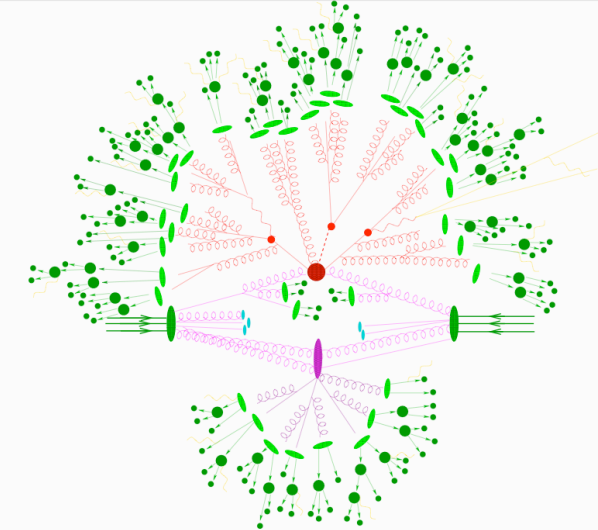
\includegraphics[width=\textwidth]{proton-to-detector}
            \end{tcolorbox}
        \end{column}
    \end{columns}
\end{frame}

\begin{frame}{Soft to Hard Physics}
    \begin{columns}
        \begin{column}{0.5\textwidth}
            \begin{figure}
                \centering
                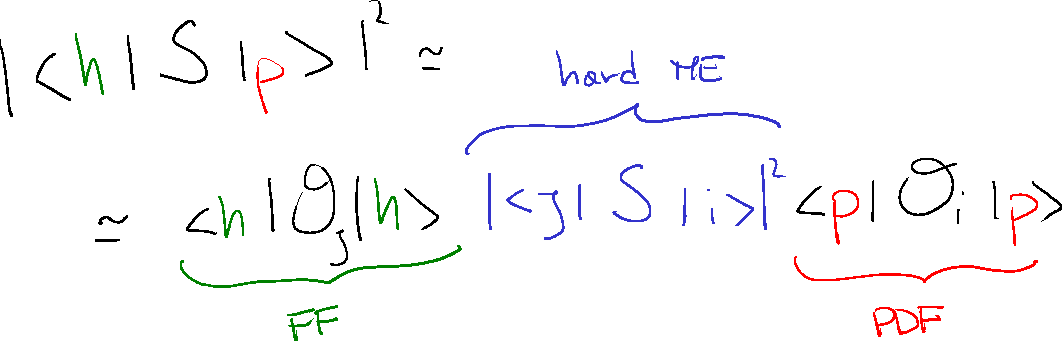
\includegraphics[width=0.9\textwidth]{hadronic-obs}
                \vspace*{10pt}
                \caption{
                    Scattering Matrix element, $\mathcal{S}$.
                    {
                        \footnotesize Fragmentation Functions only relevant for
                        non-outgoing inclusive processes.\newline
                        The operator $\mathcal{O}_i$ is essentially a number
                        operator for parton $i$, with a Wilson line (time-like
                        path) insertion for gauge covariance.
                    }
                }
            \end{figure}
        \end{column}
        \begin{column}{0.5\textwidth}
            Since QCD is non-perturbative at low energies, there is something
            \textbf{special} about \textbf{hadrons}: \textbf{we are almost
            \textit{guessing in the wild}}\footnote{
                Actually, this is a very very poor statement: we have
                constraints about theory symmetries, and the bound state net
                content. But what we \textbf{do not know} from theory is the
                \textbf{\alert{detailed structure}}, and \textbf{we need it} to
                \textit{\textbf{predict experiments}}.
            }.
            \vspace*{15pt}

            Fortunately, there is also something very \textbf{special} about
            our \textbf{theory}, and the breakdown we described: they
            \alert{\textbf{factorize}} (up to controlled sub-leading terms).
            \vspace*{15pt}

            Then we are left with our unknown non-perturbative physics, but
            nicely packaged in some \textbf{\textit{descriptive functions}},
            the \textbf{\alert{Parton Distribution Functions} (PDFs)}.
            \vspace*{25pt}
        \end{column}
    \end{columns}
\end{frame}

\begin{frame}{Target Object}
    \begin{columns}
        \begin{column}{0.5\textwidth}
            \pdf{}s then are just a set of \textbf{unknown functions}:
            \begin{equation*}
                f_i: [0, 1] \to \mathbb{R}
            \end{equation*}
            \vspace*{10pt}

            There is one for each flavor $i$, and they obey some
            \textit{theoretical constraints} (e.g.\ number and momentum sum
            rules, constraining the integral).
        \end{column}
        \begin{column}{0.5\textwidth}
            \begin{tcolorbox}
                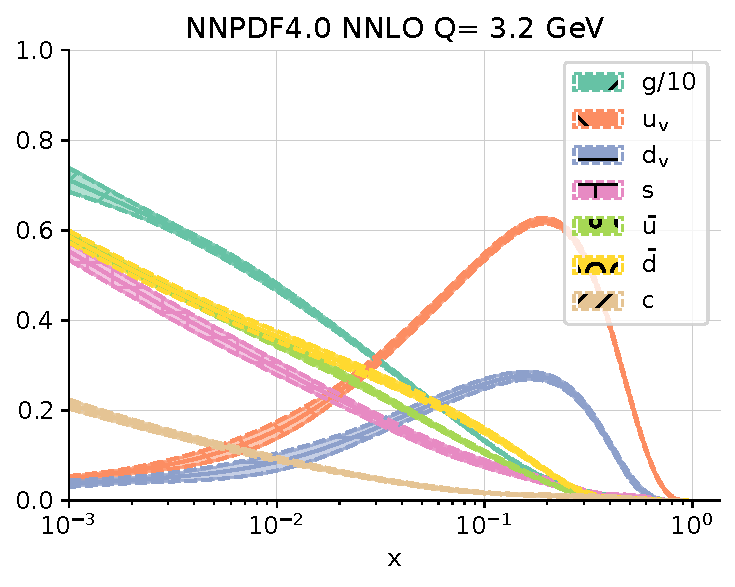
\includegraphics[width=\textwidth]{pdfs_pdg_Qs0_plot_flavours}
            \end{tcolorbox}
        \end{column}
    \end{columns}
\end{frame}

\section{Inverse Problem}

\begin{frame}{Direct problem}
    \begin{columns}
        \begin{column}{0.7\textwidth}
            \begin{figure}
                \centering
                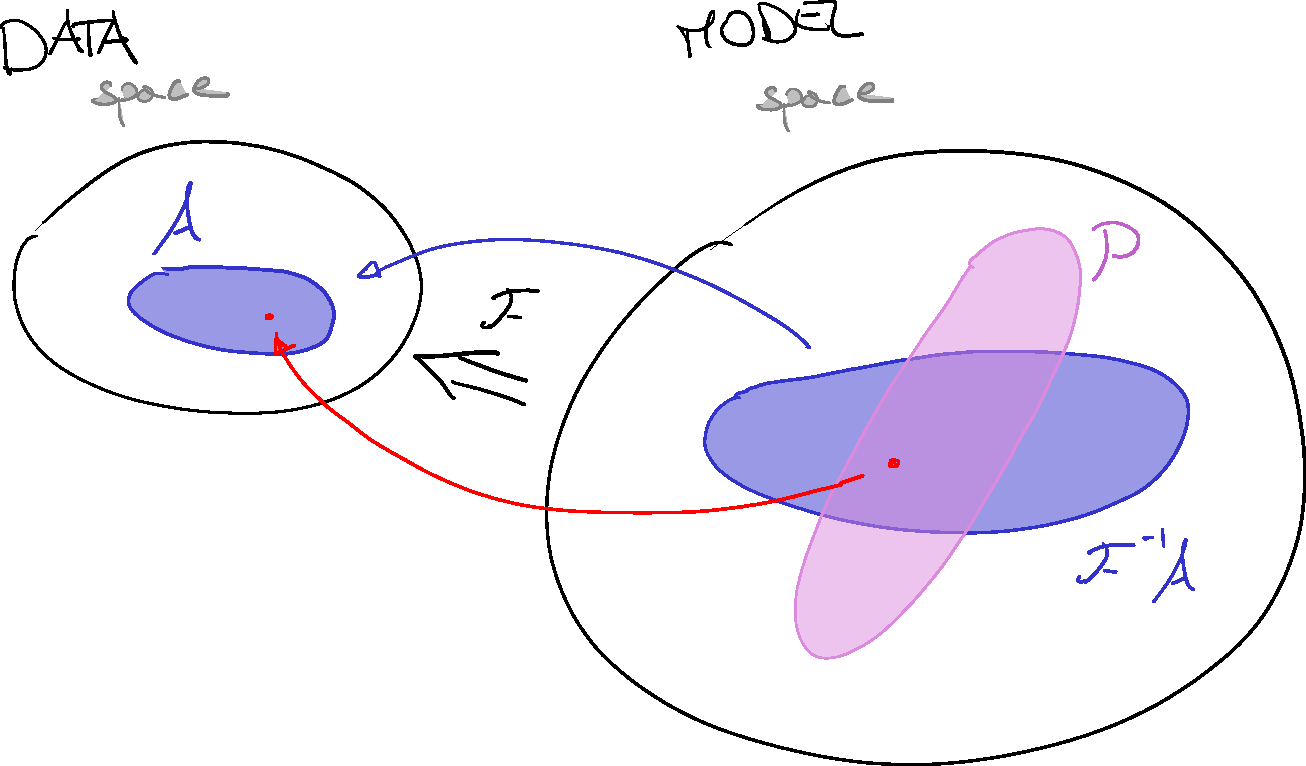
\includegraphics[width=0.8\textwidth]{inverse-problem}
                \vspace*{15pt}
                \caption{
                    The map $\mathcal{F}$ transform the model into data.
                    $\mathcal{P}$ is the parametrization space.
                }
            \end{figure}
        \end{column}
        \begin{column}{0.3\textwidth}
            \begin{center}
                \itshape No direct observation of samples of unknown objects.
            \end{center}

            The observed objects are obtained from the unknown ones through a
            \textbf{singular transformation} (non-bijective)\footnote{
                Trivial, because function space is infinite-dimensional, while
                observed objects are finite (samples, and then even more
                \textit{\enquote{kinds}}).
            }.
            \vspace*{10pt}

            Our \textbf{inference} will then follow the opposite direction,
            that is why it is called the \alert{\textbf{inverse problem}}.
            \vspace*{15pt}
        \end{column}
    \end{columns}
\end{frame}

\begin{frame}{Theory Predictions}
    \begin{center}
        So, \alert{\textbf{which is the map}} from \textbf{\pdf} (a.k.a.\
        \textit{the object to be determined}) to the \textbf{experimental
        data}?
    \end{center}
    \vspace*{20pt}

    \begin{columns}
        \begin{column}{0.5\textwidth}
            Physics, i.e. \alert{\textbf{perturbative QCD}}:
            \begin{equation*}
                \sigma(x, Q^2) = \hat{\sigma}_{ij} \otimes f_i \otimes f_j =
                \int \dd z_1 \dd z_2 ~\hat{\sigma}(z_1, z_2, Q^2)~~
                f_i\left(\frac{x}{z_1}, Q^2\right) f_i\left(\frac{x}{z_2},
                Q^2\right)
            \end{equation*}

            \begin{description}
                \item[DGLAP evolution] integro-differential equation,
                    determining \pdf{}s at all scales from a border condition
                    at a given scale $Q_0^2$
                \item[hard cross section] short distance physics, computed
                    diagrammatically (possibly supplemented with resummation)
            \end{description}

            \vspace*{20pt}
            Since we can compute everything else\footnote{For inclusive final
            states.}, we are left with the determination of the
            \alert{\textbf{border condition}} only:
            \begin{equation*}
                f_i(x, Q_0^2)
            \end{equation*}
            \vspace*{5pt}
        \end{column}
        \begin{column}{0.5\textwidth}
            picture of evolution + hard cross section:
            \begin{itemize}
                \item \pdf at the bottom
                \item evolve upwards (with thresholds)
                \item collision at the top edge
            \end{itemize}
            repeat it for two columns at different heights
        \end{column}
    \end{columns}
\end{frame}

\begin{frame}{FK tables}
    \vspace*{20pt}
    \begin{columns}
        \begin{column}{0.5\textwidth}
            \begin{figure}
                \centering
                
\includegraphics[width=0.5\textwidth]{eko}
                \caption*{DGLAP evolution framework}
            \end{figure}
            \vspace*{10pt}

            \begin{figure}
                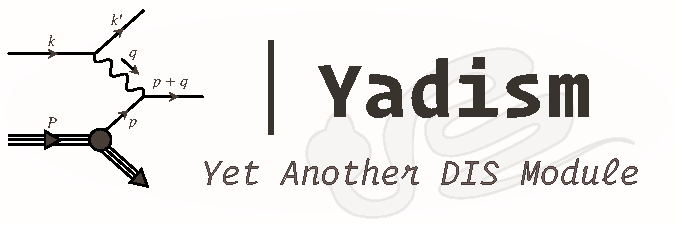
\includegraphics[width=0.7\textwidth]{yadism}
                \caption*{DIS predictions module}
            \end{figure}
            \vspace*{10pt}

            \begin{figure}
                {\Huge \textbf{PineAPPL}}
                \caption*{General process, \pdf-independent, grid storage}
            \end{figure}
        \end{column}
        \begin{column}{0.5\textwidth}
            Since we want to go through minimization, it is crucial to have a
            \textbf{fast map} from \textit{model space} to \textit{data space}:
            \begin{equation*}
                f_0(x) = f(x, Q_0^2) \to \sigma_a(x, Q^2) = \hat{\sigma}_a(Q^2)
                \otimes f(Q^2) \otimes f(Q^2)
            \end{equation*}
            \vspace*{5pt}

            We call such maps \alert{\textbf{Fast Kernel (FK) tables}}:
            \begin{equation*}
                \begin{cases}
                    F_a = FK_{a, i \alpha}~f_{0, i \alpha}\\
                    \sigma_b = FK_{b, j \beta k \gamma}~f_{0, j \beta}~f_{0, k \gamma}\\
                \end{cases}
            \end{equation*}
            since data are either \textit{linear} (one initial proton) or \textit{quadratic} (two
            protons collision) in the \pdf.\newline
            Plus \textit{composite observables} (e.g.\ ratios).

            \vspace*{15pt}
            \hrule
            \vspace*{15pt}

            For people that are familiar with perturbation theory and \pdf
            nomenclature:\newline
            when a \pdf is told to be \lo, \nlo, \nnlo, or \nnnlo, this
            is the \textit{\textbf{underlying theory order}} (the
            \texttt{FkTable}).
        \end{column}
    \end{columns}
\end{frame}

\begin{frame}{Function space}
    \begin{columns}
        \begin{column}{0.5\textwidth}
            A function $f: \mathbb{R} \to \mathbb{R}$ (or suitable intervals)
            lives in an infinite-dimensional space.
            \vspace*{20pt}

            This has a simple consequence:
            \begin{block}{Under-determination}
                Fitting an \textbf{unknown function} on a finite number of data
                is always an \textbf{under-determined} problem.
            \end{block}
            \vspace*{20pt}

            How to choose a solution, when \alert{many} are available and
            \alert{equivalent}?
        \end{column}
        \begin{column}{0.5\textwidth}
            \begin{figure}
                \centering
                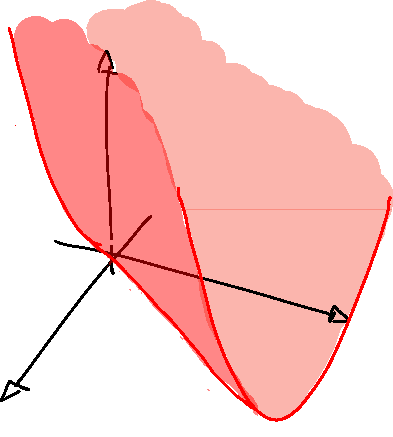
\includegraphics[width=0.6\textwidth]{underdetermined}
                \caption{Possible $\chi^2$ profile in 2D parameter space.}
            \end{figure}
        \end{column}
    \end{columns}
\end{frame}

\begin{frame}{Solutions in the Assumptions}
    \vspace*{10pt}
    \begin{center}
        There are two main ways to attack the problem.
    \end{center}
    \vspace*{10pt}

    \begin{columns}
        \begin{column}{0.5\textwidth}
            1. One consists in \textit{reducing the number of parameters}, by
            \textbf{slicing} a suitable \textbf{hyperplane}.
            \footnote{Not containing zero-directions.}
            \vspace*{10pt}

            This is what we do in PDFs when choosing a \alert{\textbf{fixed
            parametrization}}: we decide which parameters to fit, and take a
            single given value for everything else.
            \vspace*{10pt}

            \begin{figure}
                \centering
                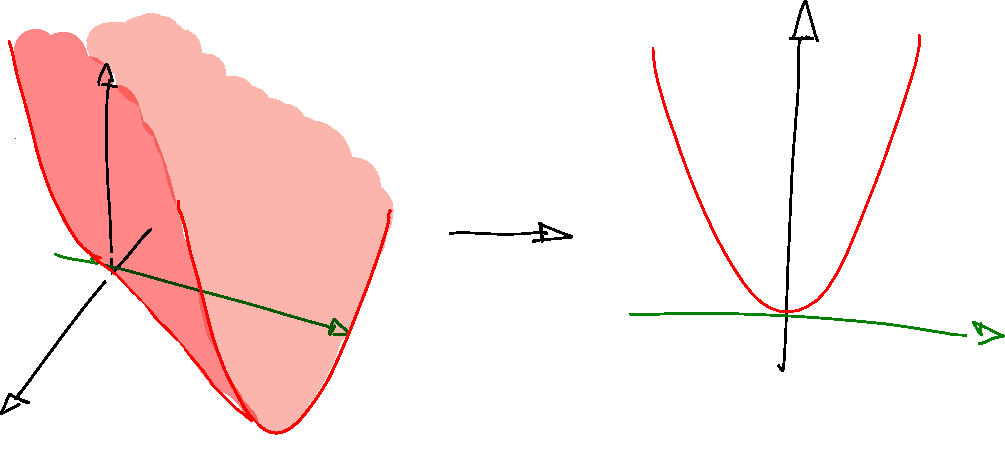
\includegraphics[width=0.8\textwidth]{sliced}
                \caption{$\chi^2$ profile in sliced parameter space.}
            \end{figure}
            \vspace*{10pt}
        \end{column}
        \begin{column}{0.5\textwidth}
            2. The second approach removes the zero-direction by adding
            \textbf{regularization}.
            \vspace*{10pt}

            This is what the \alert{\textbf{Neural Network}} (and its training
            algorithm) is doing under the hood.
            \vspace*{10pt}

            \begin{figure}
                \centering
                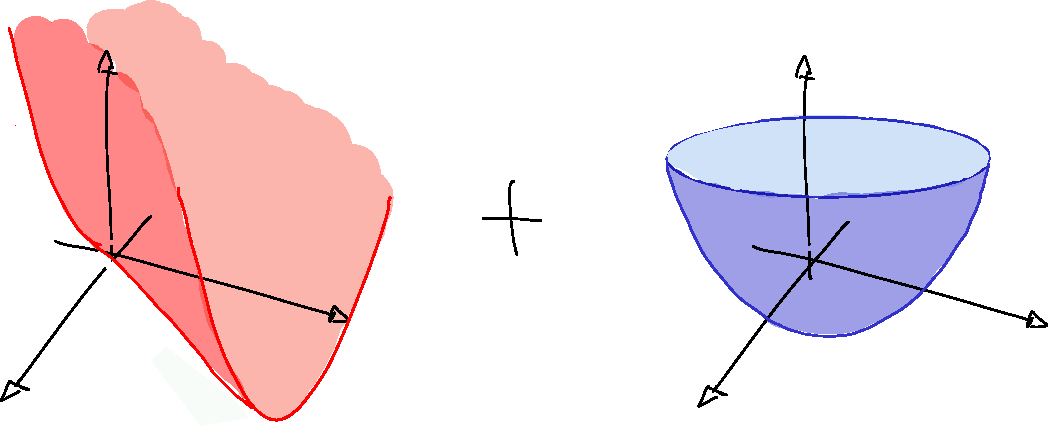
\includegraphics[width=0.8\textwidth]{regularized}
                \caption{$\chi^2$ profile plus regularization function.}
            \end{figure}
        \end{column}
    \end{columns}
\end{frame}

\begin{frame}{So Which?}
    \vspace*{15pt}
    \begin{columns}
        \begin{column}{0.5\textwidth}
            Then which one should we choose?
            \vspace*{10pt}

            \begin{figure}
                \centering
                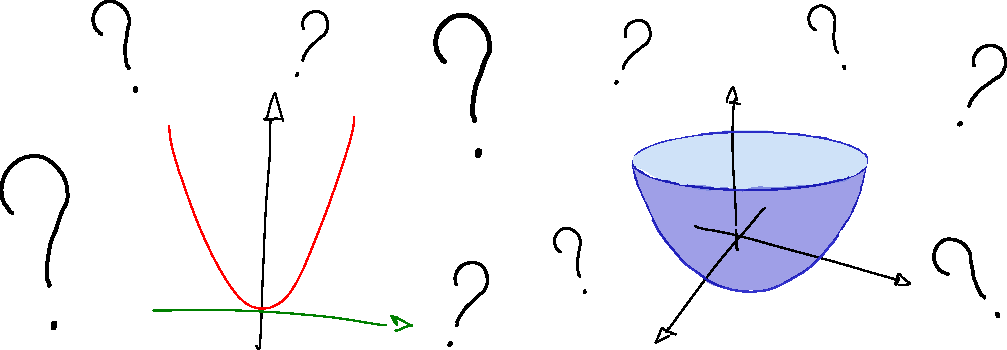
\includegraphics[width=0.9\textwidth]{choice}
            \end{figure}

            \vspace*{10pt}
            There is \textbf{not} an \alert{\textbf{absolute best answer}},
            because both procedures might be \textit{\textbf{arbitrary}}.
        \end{column}
        \begin{column}{0.5\textwidth}
            In need for guiding principle to make a good choice, proposal:
            \vspace*{-2pt}
            \begin{center}
                \itshape
                \bfseries
                Choices should encode physics assumptions
            \end{center}
            \vspace*{-2pt}
            and as little arbitrariness as possible\footnote{
                Though nothing is actually bias-free, so better to know and
                declare your bias, rather than hiding it.
            }.

            \vspace*{15pt}
            So what about PDFs?
            \begin{description}
                \item[cuts] cutting the space (fixed parametrization) is no
                    bad, \textbf{if you know how to do it}: you need
                    \alert{\textbf{precise theoretical insight}} on the
                    \alert{\textbf{\pdf shape}}
                \item[regularization] also this need as much motivation as the
                    former, but it makes \textit{to shift the focus} from the
                    exact shape to more abstract \alert{\textbf{features}}
            \end{description}
            \vspace*{5pt}
        \end{column}
    \end{columns}
    \vspace*{10pt}

    \begin{center}
        
\includegraphics[width=2.5cm]{../_logos/nnpdf_logo.pdf} approach $\to$
        use a \textbf{Neural Network as the \alert{representation} for the
        unknown function}.
    \end{center}
    \vspace*{10pt}

    Notice that usually a NN is used to perform a task. Here the NN is actually
    representing the unknown object itself.\newline
    \vspace*{-2pt}
    {\footnotesize
        \hspace*{-5pt}
        I.e., usually, evaluate on your input once, to obtain the candidate
        output. Here, many evaluation of the same network on an array of inputs
        needed to perform the same task.
    }
\end{frame}

\section{Uncertainties = Distribution}

\begin{frame}{Propagating Error}
    \begin{columns}
        \begin{column}{0.5\textwidth}
            \begin{figure}
                \centering
                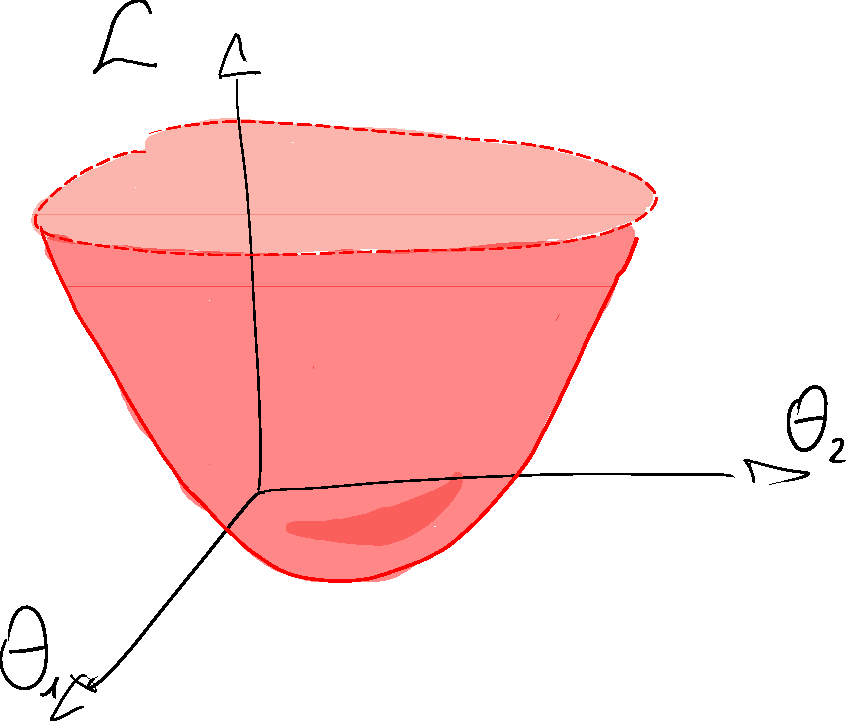
\includegraphics[width=0.6\textwidth]{hessian}
                \caption*{
                    Usually the Hessian is used together with the $\chi^2$ as
                    loss.
                }
            \end{figure}
        \end{column}
        \begin{column}{0.5\textwidth}
            The Hessian approach is possibly the simplest: essentially, relies
            on a quadratic approximation of the loss function near the minimum
            (\textit{best fit}) $\hookrightarrow$ Gaussian distribution in
            parameter space.
            \vspace*{10pt}

            So, given a restricted set of parameters, the determination of the
            multi-Gaussian relies on:
            \begin{description}
                \item[eigenvectors] as eigenvectors of the loss itself
                \item[variance] variances, derived from inverse loss curvature
            \end{description}
            \vspace*{10pt}

            So the distribution resembles:
            \begin{equation*}
                P(\theta | \mathcal{D}) = \exp(-\chi^2(\theta; \mathcal{D}))
            \end{equation*}
        \end{column}
    \end{columns}
    
\end{frame}

\begin{frame}{Replicas}
    \nnpdf{} Approach

    Na\"ive idea: the error comes from data, let's propagate the data
    distribution back through the \textit{inverse function}:
    \begin{equation*}
        \mathcal{F}(D) = \argmin_\theta\left(\mathcal{L}(D)\right)
    \end{equation*}

    Maybe insert one of the usual methodology diagram, to fill space (or hand
    draw it).
\end{frame}

\begin{frame}{The NN}
    \begin{center}
        What is then doing the neural network (NN)? Why is it working so well?
    \end{center}
    \vspace*{10pt}

    \begin{columns}
        \begin{column}{0.5\textwidth}
            \begin{figure}
                \centering
                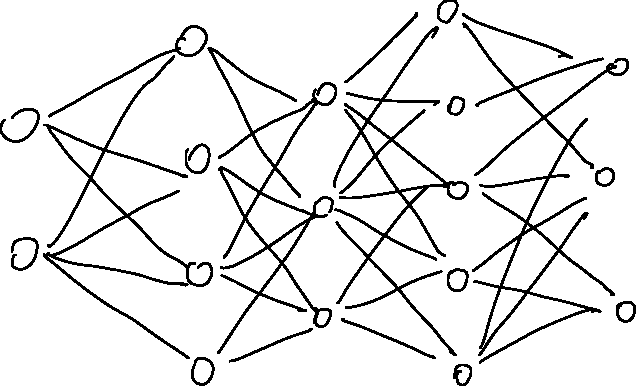
\includegraphics[width=0.6\textwidth]{nn}
            \end{figure}

            \vspace*{10pt}
                Essentially, the \textit{NN is encoding} an
                \alert{\textbf{interpolation hypothesis}} \textit{in the
                architecture \textbf{and} training algorithm}.
        \end{column}
        \begin{column}{0.5\textwidth}
            While both the approaches are limiting \textit{model complexity},
            the \textbf{Neural Network} is free enough to follow strong
            \textbf{data trends}.

            \vspace*{10pt}
            \begin{exampleblock}{Physical Wiggles}
                A criticism we collected has been about \textit{NN opaque
                assumptions} might \textbf{prevent} to follow \textbf{small
                physical fluctuations}, but it is actually the other way
                round:\footnote{In principle, yet to be proven in practice.}

                \begin{description}
                    \item[fixed param.] in this case, you can only find
                        oscillations you are allowing for, so you need to know
                        in advance \textbf{each and every wiggle} to
                        discriminate physical ones from noise
                    \item[NN] all wiggles are deweighted, but physical wiggles
                        should be resolved more and more by data, so
                        \textit{"enough precision"} in the
                        \alert{\textbf{data}} will naturally
                        \textbf{\alert{overwhelm} the theoretical
                        \alert{(learning) bias}}
                \end{description}
            \end{exampleblock}
        \end{column}
    \end{columns}
\end{frame}

\begin{frame}{Propagating Error}
    \nnpdf{} Approach - reinterpreted
    \footnotetext{
        \paperref{https://doi.org/10.1140/epjc/s10052-022-10297-x}{\textit{L. Del
        Debbio, T. Giani, M. Wilson}, Eur.Phys.J.C 82 (2022) 4, 330}
    }. (Luigi's paper)

    Hints for a better approach (if it's equivalent to something meaningful,
    maybe it would be worth to try that something).

    
\end{frame}

\section{Trust the Results}

\begin{frame}{Dataset}
    \vspace*{5pt}
    As physicists, we \alert{\textbf{trust in data}} (physics $\sim$
    experimental science).
    \begin{center}
        \begin{tcolorbox}[width=0.65\textwidth]
            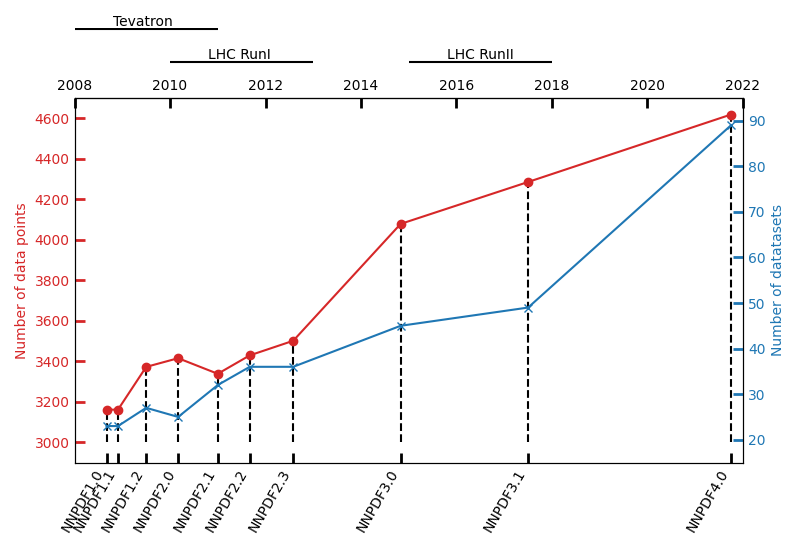
\includegraphics[width=\textwidth]{data}
        \end{tcolorbox}
    \end{center}
    \textbf{Variety} of datasets, to \textbf{cover different features} of the
    \textit{underlying object}.
\end{frame}

\begin{frame}{Amazing Black Box}
    What happens when you don't trust NN?
    \begin{columns}
        \begin{column}{0.5\textwidth}
            Common criticism is the NN being a black box
        \end{column}
        \begin{column}{0.5\textwidth}
            \begin{figure}
                \centering
                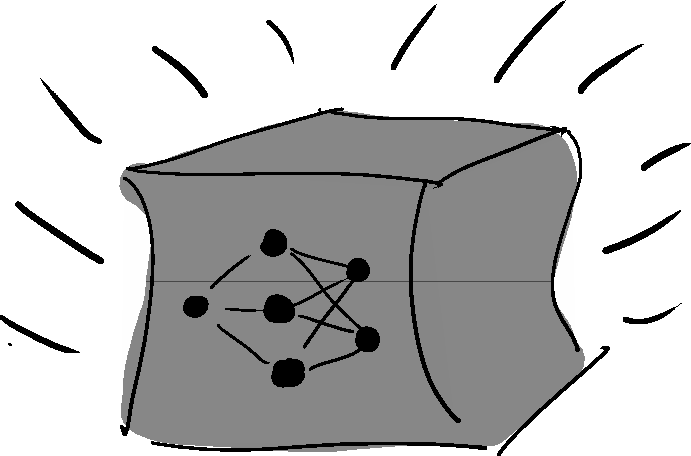
\includegraphics[width=0.7\textwidth]{black-box}
            \end{figure}
        \end{column}
    \end{columns}
\end{frame}

\begin{frame}{Closure Tests}
    Controls data region.
    \begin{columns}
        \begin{column}{0.5\textwidth}
            \begin{figure}
                \hspace*{20pt}
                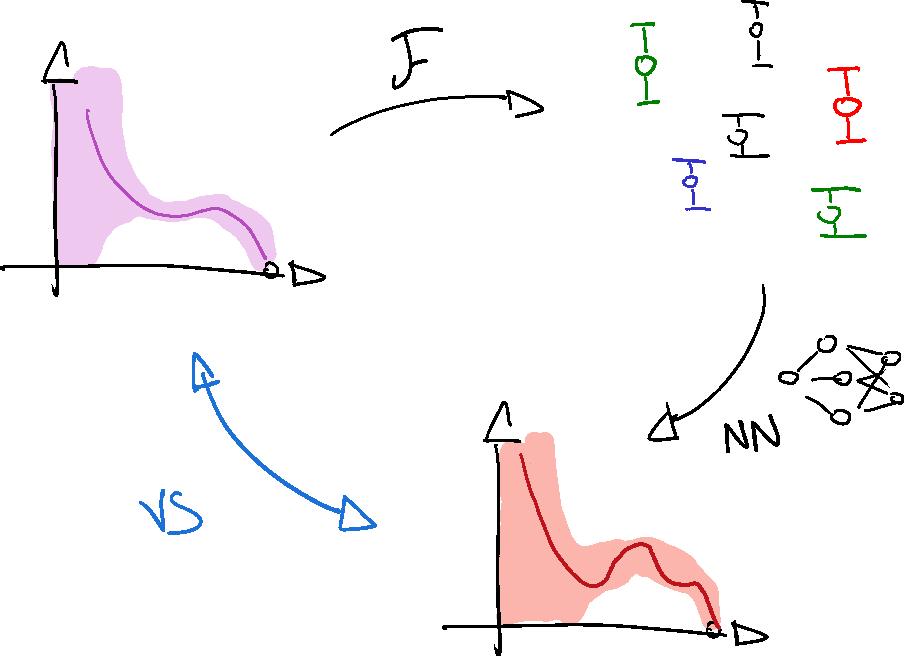
\includegraphics[width=0.9\textwidth]{closure-tests}
            \end{figure}
        \end{column}
        \begin{column}{0.5\textwidth}
            \begin{description}
                \item[Level 0] generate data from \textbf{\enquote{true}
                    central value} only: $\chi^2_{expected} \sim 0$
                    {\footnotesize (essentially: can we find that central
                    value? Is it forbidden?)}
                \item[Level 1] generate data from the \textbf{\enquote{true}
                    distribution} $\chi^2_{expected} \sim 1$
                    {\footnotesize a \enquote{usual} distribution
                    determination}
                \item[Level 2] Add \textbf{pseudo-data} generation,
                    $\chi^2_{expected} \sim 2$
            \end{description}
            \vspace*{20pt}
            
            Too large errors and too small are both wrong, almost the same as
            missing the central value.
            {\footnotesize (unless being able to prove to consistently
            over-estimate, without being able to compute it to subtract)}
        \end{column}
    \end{columns}
    \vspace*{20pt}

    Experimental data are far from perfect, they might be affected by several
    inconsinstencies.
    \begin{flushright}
        $\to$ model inconsinstencies in the data generation process, a.k.a.\
        \enquote{closure test with inconsistent data}, WIP
    \end{flushright}
\end{frame}

\begin{frame}{Future Tests}
    Controls extrapolation region: what about data you have not seen yet?
    \vspace*{10pt}

    \begin{figure}
        \centering
        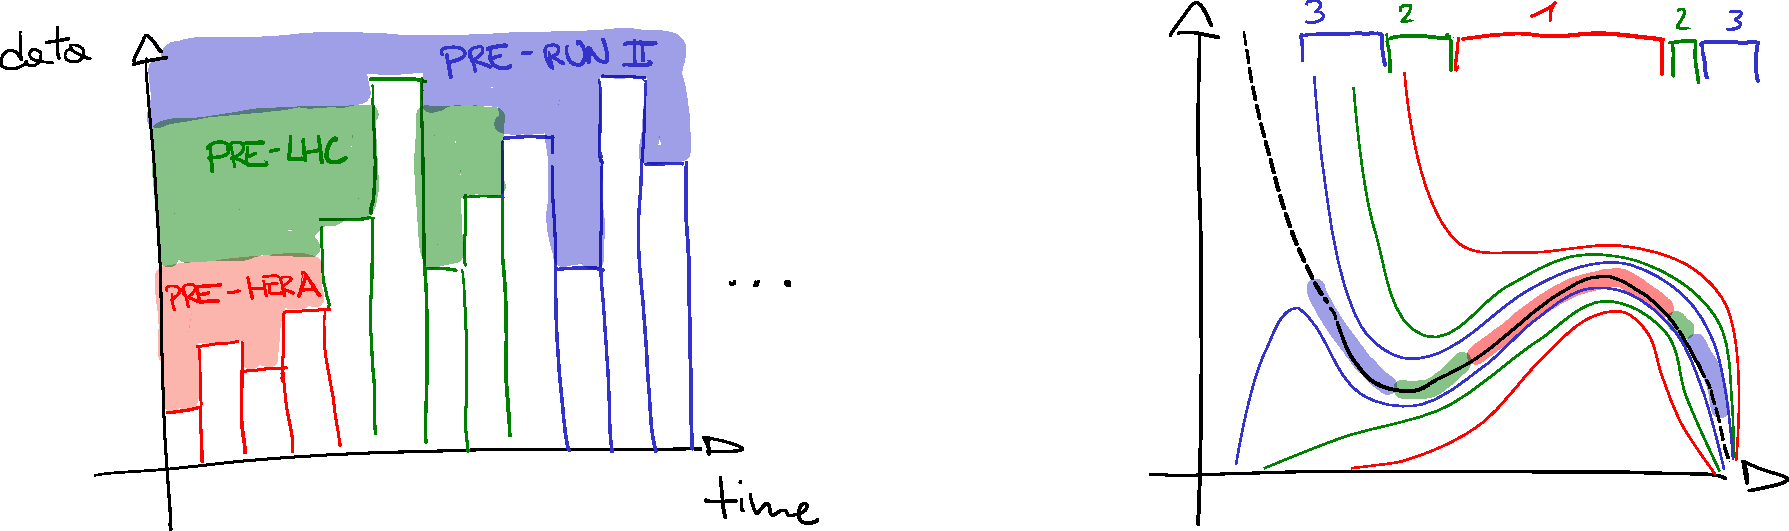
\includegraphics[width=0.8\textwidth]{future-tests}
    \end{figure}

    Well, I can not travel to the future, but I know history, and I can set my
    fiction in a past scenario :)
    (not like a full blind analysis, my prior knows about \enquote{the future},
    but it is a further consistency check)
\end{frame}

\section{Results}

\begin{frame}{Uncertainties - Data Region}
    \begin{columns}
        \begin{column}{0.5\textwidth}
            \vspace*{10pt}

            Here, the result of the \textbf{\textit{\enquote{Physical
            Wiggles}}} issue is evident: in order to nicely fit result with a
            rather \textbf{restrictive parametrization}, you need to inflate
            your errors (\textit{\alert{\textbf{tolerance}} procedure}).
            \vspace*{15pt}

            However, keep in mind that \nnpdf{4.0} has a \textit{wider
            datasets} then the other releases.\newline
            Implementing data has a non-trivial retrieval and interpretation
            cost (lack of standard language, especially for systematics), plus
            theory implementation (the \texttt{FkTable}).
            \vspace*{15pt}

            But \nnpdf{3.1} has already smaller uncertainties than more recent
            releases, e.g.\ \texttt{CT18} and \texttt{MSHT18}, despite a
            slightly smaller\footnote{Disputable.} dataset.\newline
            This is the \alert{\textbf{methodology impact}}.
            \vspace*{15pt}
        \end{column}
        \begin{column}{0.5\textwidth}
            \begin{tcolorbox}
                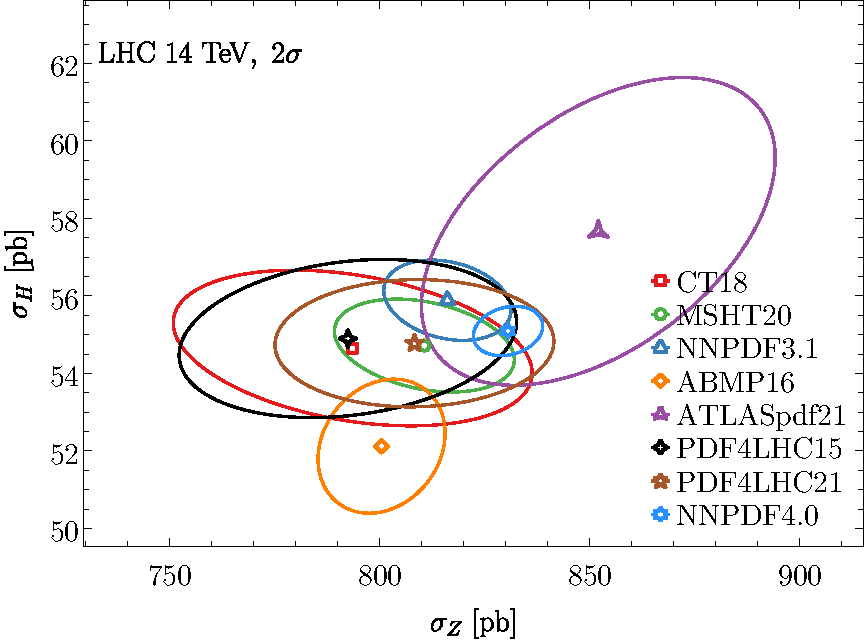
\includegraphics[width=\textwidth]{Corr_Z2H14TeV_2sigma}
            \end{tcolorbox}
        \end{column}
    \end{columns}
\end{frame}

\begin{frame}{Uncertainties - Extrapolation - Large $x$}
    \begin{columns}
        \begin{column}{0.5\textwidth}
            \begin{tcolorbox}[size=small,sharpish corners,boxrule=0mm]
                \centering
                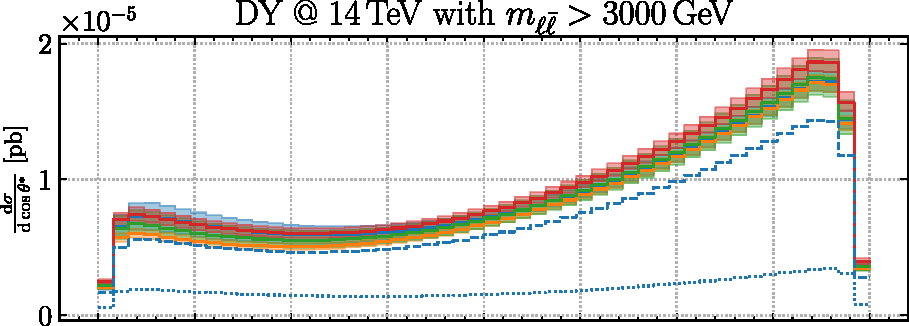
\includegraphics[width=0.49\textwidth]{NNPDF_DY_14TEV_BSM_AFB_COS_3000}
                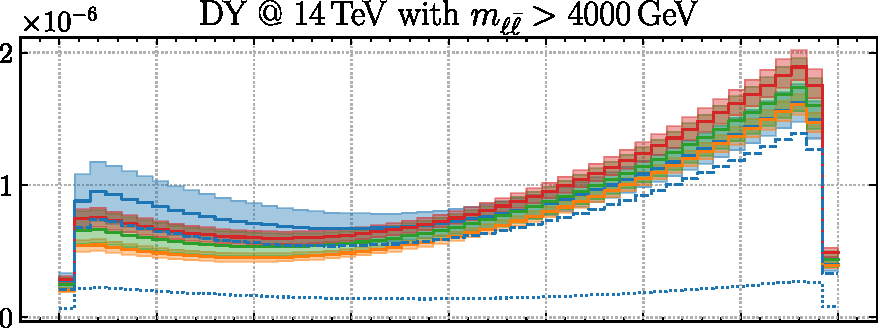
\includegraphics[width=0.49\textwidth]{NNPDF_DY_14TEV_BSM_AFB_COS_4000}
            \end{tcolorbox}
            \vspace*{20pt}

            Rather biased result \textbf{encoded} in the \textbf{hypothesis}:
            the large invariant mass extrapolation region maps to the large-$x$
            behavior of the \pdf{}, that is \textit{\textbf{little constrained
            by data}}.
            But a fixed parametrization propagate the behavior of the data
            region.
            \vspace*{10pt}

            While \nnpdf{4.0} has very \textbf{\textit{small uncertainties}} in
            the \textbf{\textit{data region}}, it is still flexible enough to
            \textbf{inflate in extrapolation}, encoding the \alert{\textbf{lack
            of experimental knowledge}}.
            \vspace*{20pt}


            \begin{tcolorbox}[size=small,sharpish corners,boxrule=0mm]
                \centering
                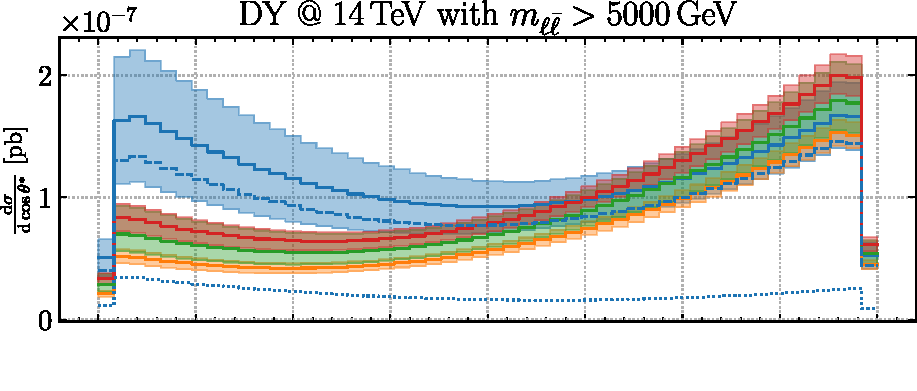
\includegraphics[width=0.49\textwidth]{NNPDF_DY_14TEV_BSM_AFB_COS_5000}
                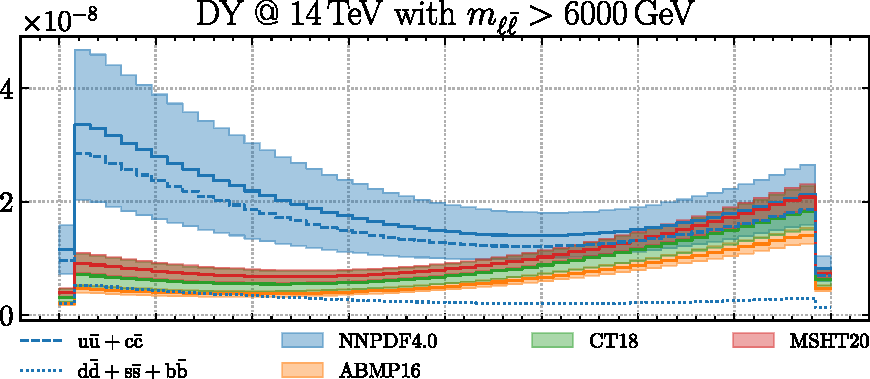
\includegraphics[width=0.49\textwidth]{NNPDF_DY_14TEV_BSM_AFB_COS_6000}
            \end{tcolorbox}
        \end{column}
        \begin{column}{0.5\textwidth}
            \begin{tcolorbox}
                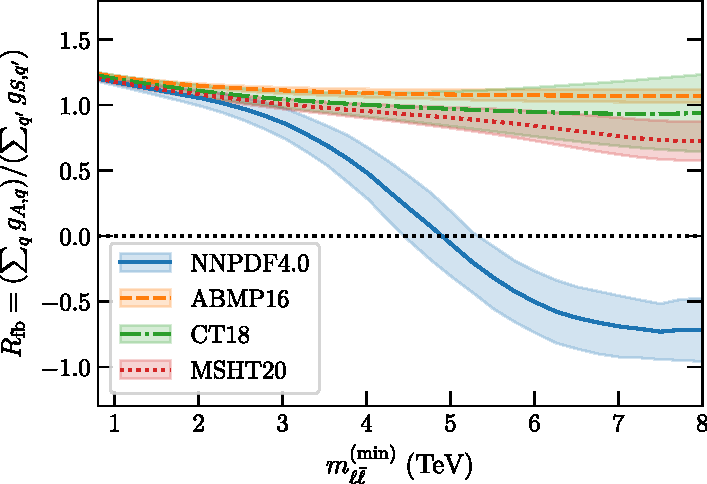
\includegraphics[width=\textwidth]{asym_coeff_mlldep}
            \end{tcolorbox}
        \end{column}
    \end{columns}
\end{frame}

\begin{frame}{Intrinsic Charm}
    \vspace*{-15pt}
    \begin{center}
        $3\sigma$ of an \textbf{intrinsic} (non-perturbative)
        \textbf{\alert{charm} component} of the \textbf{proton}.

        \paperref{https://doi.org/10.1038/s41586-022-04998-2}{Nature 608 (2022)
        7923, 483-487}
    \end{center}
    \vspace*{15pt}

    \begin{columns}
        \begin{column}{0.5\textwidth}
            \begin{tcolorbox}
                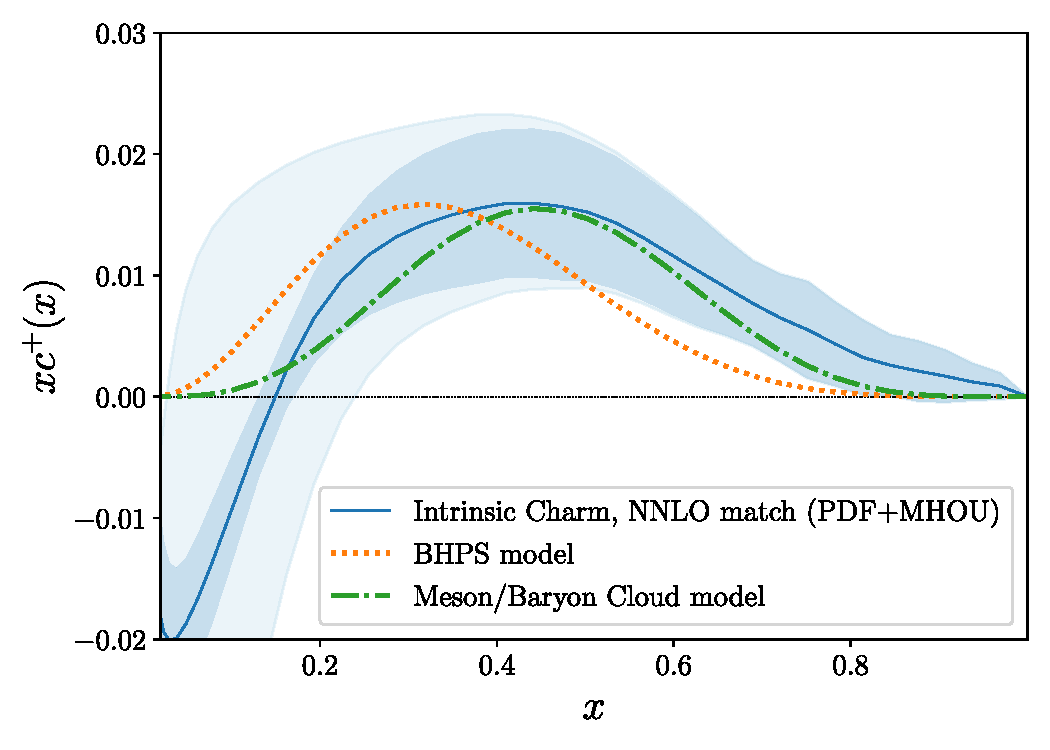
\includegraphics[width=\textwidth]{nf3_to_models}
            \end{tcolorbox}
        \end{column}
        \begin{column}{0.5\textwidth}
            \begin{tcolorbox}
                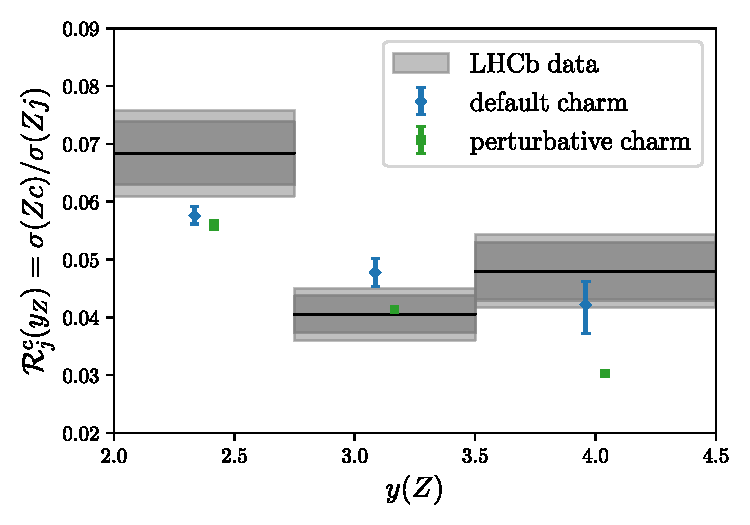
\includegraphics[width=\textwidth]{lhcb-zcharm-pheno}
            \end{tcolorbox}
        \end{column}
    \end{columns}
\end{frame}

\section{Conclusions}

\begin{frame}{Summary}
    \vspace*{15pt}

    Title question: \textit{\enquote{How to learn a function?}}
    \vspace*{10pt}

    \begin{columns}
        \begin{column}{-0.05\textwidth}
        \end{column}
        \begin{column}{0.45\textwidth}
            \begin{enumerate}
                \item Reduce to a \alert{\textbf{finite} problem} through soft
                    but \textbf{sensible assumptions} (e.g.\ interpolation)
                \item \alert{Minimize \textbf{suitable loss}} function in data
                    space, including \textbf{extra constraints} (usually
                    theoretical knowledge)
                \item Apply an \alert{\textit{\enquote{error propagation}}}
                    technique (\textbf{posterior determination/sampling})
                \item \alert{\textbf{Test}} over and over your methodology
                    (empirical robustness proof, i.e.\ consistency check)
            \end{enumerate}
        \end{column}
        \begin{column}{0.45\textwidth}
            In this way, it is possible to learn a lot!
            \vspace*{10pt}
            
            But we actually have little to poor insight on \textit{\enquote{why
            is my inference working?}}. And thus \textit{\enquote{Is it
            actually working?}}
            \vspace*{10pt}

            Good scientists are \uline{\textbf{skeptic} of their own results},
            but we still need to \alert{\textit{act to the best of our
            options}}, while preserving \textbf{caution}.
        \end{column}
    \end{columns}
    \vspace*{-10pt}

    \begin{columns}
        \begin{column}{0.65\textwidth}
            But: is a Neural Network really \textbf{the best tool} for this
            kind of tasks?
            \vspace*{10pt}

            \hspace*{20pt}\textbf{Next Episode}
            {\footnotesize (\textit{clue above $\hookuparrow$:
            \textbf{posterior sampling}})}
        \end{column}
        \begin{column}{0.25\textwidth}
            \hspace*{-10pt}
            
\includegraphics[width=0.5\textwidth]{skeptic}
        \end{column}
    \end{columns}
\end{frame}

\begin{frame}{Tools and References}
    \begin{columns}
        \begin{column}{0.5\textwidth}
            \uline{{\LARGE\itshape Collaboration and references}}
            \vspace*{15pt}

            For all info about the collaboration, cf.:

            \begin{center}\url{https://nnpdf.mi.infn.it}\end{center}

            including talks, papers and code.

            \vspace*{5pt}
            \begin{figure}
                \centering
                
\includegraphics[width=2.5cm]{../_logos/nnpdf_logo.pdf}
            \end{figure}
            \vspace*{10pt}

            A few more items at:

            \begin{center}\url{https://n3pdf.mi.infn.it}\end{center}

            \vspace*{5pt}
            \begin{figure}
                \centering
                
\includegraphics[width=2.5cm]{../_logos/n3pdf_logo.pdf}
            \end{figure}
        \end{column}
        \begin{column}{0.5\textwidth}
            \uline{{\LARGE\itshape Public Code}}
            \vspace*{15pt}

            Introduction paper:\hspace*{10pt}
            \paperref{https://doi.org/10.1140/epjc/s10052-021-09747-9}{Eur.Phys.J.C 81 (2021) 10, 958}
            \vspace*{10pt}

            Code and docs:
            \vspace*{5pt}

            \hspace*{15pt}\githuburl{https://github.com/NNPDF/nnpdf}\newline
            \hspace*{15pt}\url{https://docs.nnpdf.science}

            \vspace*{10pt}
            \begin{figure}
                \centering
                
\includegraphics[width=0.15\textwidth]{tensorflow}
                \hspace*{0.25\textwidth}
                
\includegraphics[width=0.15\textwidth]{python}
            \end{figure}
        \end{column}
    \end{columns}
\end{frame}

\begin{frame}[standout]
    Thanks for your attention!
\end{frame}

\appendix

\begin{frame}{Looking for Insights}
    \begin{columns}
        \begin{column}{0.5\textwidth}
            \textit{NNPDF "framework"} is much \textbf{\textit{more}} than a Neural
            Network only:
            \begin{itemize}
                \item nice representation of a generic distribution (\textbf{replicas})
                \item many \textbf{tests} in place
                \item \textbf{fast theory} framework
                \item \textbf{lots of data} implemented
                \begin{itemize}
                    \item both theory calculation and
                    \item commondata implementation with uncertainties
                        (including correlated systematics)
                \end{itemize}
                \item and more\dots
            \end{itemize}
            \vspace*{10pt}

            \begin{center}
                \itshape
                We do \textbf{not} want to \textbf{loose} \alert{\textbf{any}} of these.
            \end{center}
        \end{column}
        \begin{column}{0.5\textwidth}
            But sometimes we \textbf{lack insight}: we have tests for this, but
            they are not always a handy tool to answer all questions.
            \vspace*{10pt}

            \begin{exampleblock}{Hopscotch}
                \begin{center}
                    \itshape
                    What are our criticism to CT replicas?
                \end{center}
                Mostly we blame the method, but little criticism on the result.

                Some \textbf{physical assumptions} have been checked:
                \begin{itemize}
                    \item $\chi^2$ vs $\chi^2_{t_0}$
                    \item integrability and sum rules
                    \item positivity
                \end{itemize}

                But it might be hidden in the NN \textbf{regularization}.
            \end{exampleblock}

        \end{column}
    \end{columns}

    \vspace*{10pt}
    Another limitation\footnote{
        Actually, this is where everything started from.
    } is that the current methodology need to make a \textbf{fit to \alert{one
    sample} at a time}. The distribution is only the result of many fits.

    \vspace*{-5pt}
    \begin{center}
        \itshape
        \bfseries
        What if we could fit the distribution all at once?
    \end{center}
    \vspace*{-10pt}
\end{frame}

\begin{frame}{Restart from Bayes}
    \begin{columns}
        \begin{column}{0.5\textwidth}
            Typical examples of ML are:
            \begin{itemize}
                \item image and speech recognition
                \item generative tasks,
                \item style transfer
                \item and so on...
            \end{itemize}
            \vspace*{10pt}

            All these problems have in common:
            \begin{center}
                very \textbf{high dimensional} objects, with
                \alert{\textbf{poor analytical/algorithmic insight}} on its
                structure.   
            \end{center}
            Working out an explicit and effective representation for them would
            be difficult.
            \vspace*{10pt}

            Not the case for \pdf{}s: \textbf{math language description} and
            \textbf{clear analytic properties} at hand (sum rules, power-like
            behavior, and so on\dots).
        \end{column}
        \begin{column}{0.5\textwidth}
            \begin{figure}
                \centering
                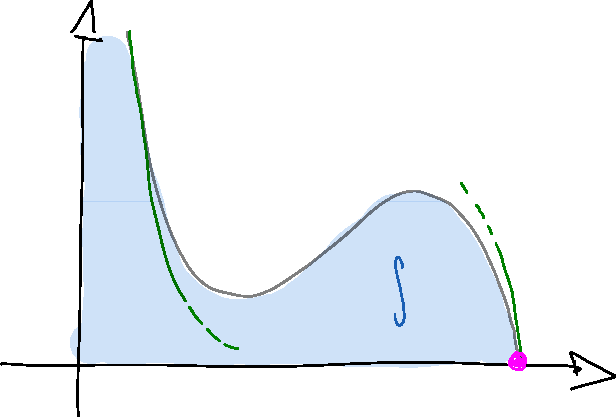
\includegraphics[width=0.6\textwidth]{pdf}
                \caption{\pdf analytical features.}
            \end{figure}

            Then, we can follow a rather simple analytical approach:
            \begin{equation*}
                P(A|B) = \frac{P(B|A) P(A)}{P(B)}
            \end{equation*}
            
            Bayes formula exposes \textbf{regularization} explicitly in the
            prior, so the assumptions are analytically transparent.
        \end{column}
    \end{columns}
\end{frame}

\begin{frame}{Prior Choice \& Implementation}
    \begin{center}
        But then the question: \textbf{\textit{which prior?}}
    \end{center}
    \begin{columns}
        \begin{column}{0.5\textwidth}
            \textbf{A:} a Gaussian process
            \begin{figure}
                \centering
                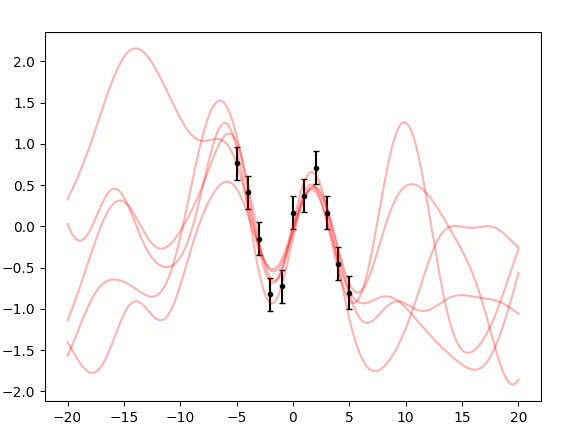
\includegraphics[width=0.9\textwidth]{sine6}
            \end{figure}

            Essentially a \textit{multi-Gaussian} with a \textbf{metric-driven
            kernel}, with the motivation that is simple, and sufficiently
            flexible.
        \end{column}
        \begin{column}{0.5\textwidth}
            Basic ideas:
            \begin{description}
                \item[parametrization] exactly our delivery: we use \pdf values
                    at grid points (we would no expose more degree of freedom
                    anyhow, so no need to use them)
                \item[transformations] data are not in the \pdf space, but we
                    can use linear and non-linear (quadratic) transformations
                \item[sum rules] the Gaussian process allow us to impose them
                    analytically (in practice, it is easier to impose them as
                    \textit{zero-error data}, but it is only a technicality)
                    \begin{itemize}
                        \item the important thing is that we can
                            \textbf{constrain integral and derivatives} as much
                            as the process, thanks to the \textit{metrical
                            kernel}
                    \end{itemize}
                \item[integrability] integrability and extrapolation behavior
                    it is implemented as constraints on hyper-parameters
                \item[positivity] we can implement as constraint on the process
            \end{description}
        \end{column}
    \end{columns}
\end{frame}


\begin{frame}{(Very) Preliminary Results}
    \vspace*{10pt}
    \begin{figure}
        \centering
        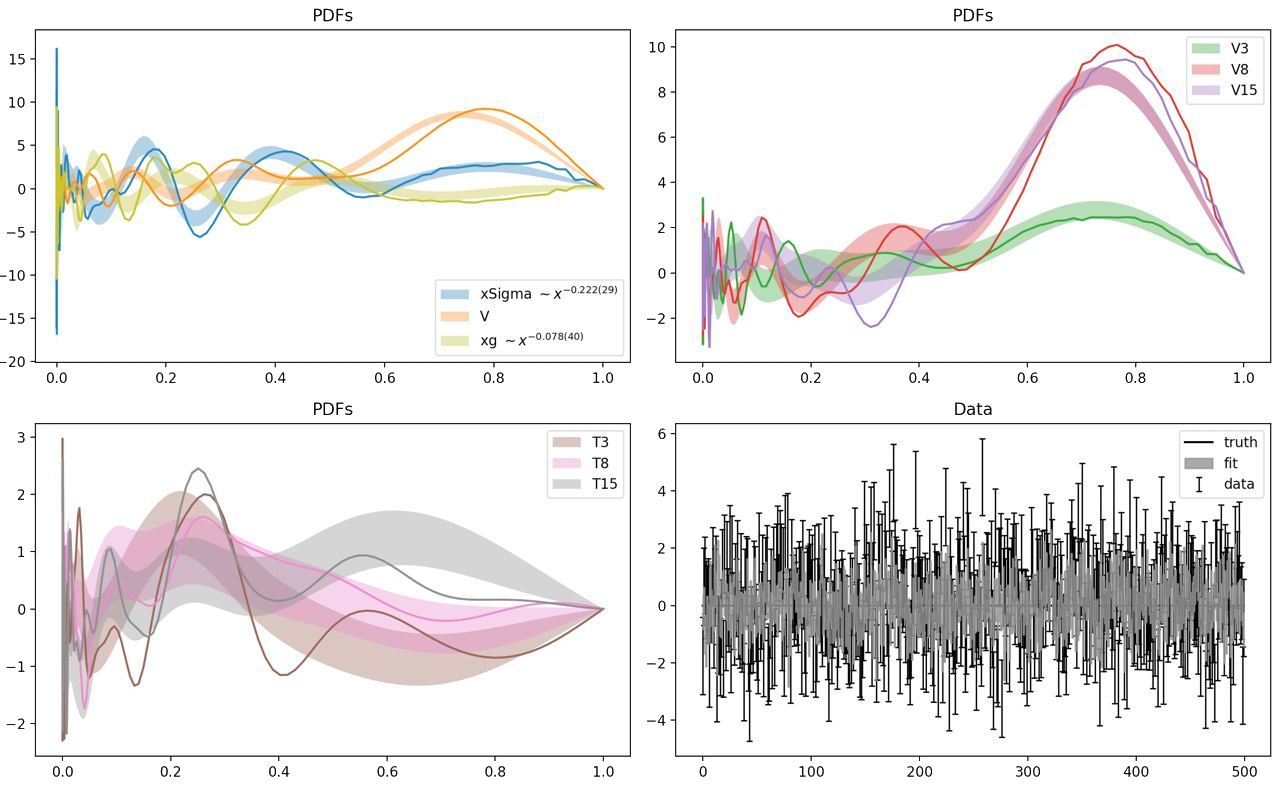
\includegraphics[width=0.75\textwidth]{fit-pdf}
        \caption{
            Even with completely random data and theory, we get a valence like
            structure (\textbf{valence peak}, wrong place, wrong height) by
            virtue of \textbf{sum rules}. Still, they are too much
            unconstrained to get correct values.
        }
    \end{figure}
\end{frame}

\begin{frame}{End of NN?}
    \begin{center}
        \itshape Can we \alert{\textbf{retire}} the \textbf{Neural Network}?
    \end{center}
    \vspace*{10pt}

    \begin{columns}
        \begin{column}{0.02\textwidth}
        \end{column}
        \begin{column}{0.6\textwidth}
            The basic, and most uninformative, answer is \textbf{\enquote{maybe}}.
            \vspace*{10pt}

            In practice, the Neural Network is doing \textit{\textbf{quite a
            good job}} at giving a \textbf{simple} enough \textbf{recipe to
            \alert{determine our kernel}}.
            $\to$ At the \textbf{price} of \textbf{insight loss}.
            \vspace*{10pt}

            It has trade-offs, but it is doing a rather good job, as proven by
            tests.
            It would be silly to completely forget about it, since it is
            providing another access path to, \textit{in principle}, equivalent
            results.
        \end{column}
        \begin{column}{0.3\textwidth}
            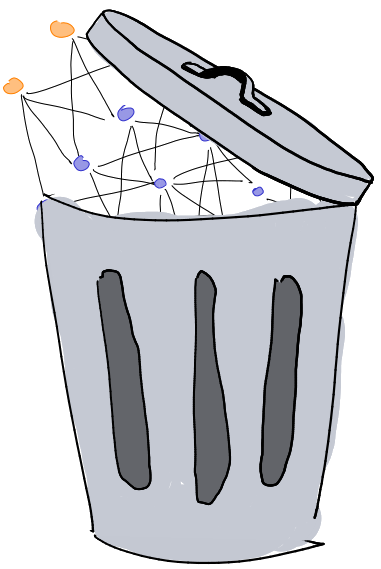
\includegraphics[width=0.8\textwidth]{retire-nn.png}
        \end{column}
    \end{columns}
\end{frame}

\begin{frame}{Hyper-opt}
    You can get the full distribution, including \textbf{hyper-parameters}:
    \begin{equation*}
        P(A|B;\lambda) = \frac{P(B|A) P(A;\lambda)}{P(B)}
    \end{equation*}

    And, \textit{if you wish}, you can \alert{\textbf{hyper-optimize}} to get a
    single value:
    \begin{equation*}
        \begin{cases}
            \lambda^* = \max_{\lambda \in \Lambda} P(A|B;\lambda)\\
            P(A|B) = \max_{\lambda \in \Lambda} P(A|B;\lambda) = P(A|B; \lambda^*)
        \end{cases}
    \end{equation*}
    
    This is just the \textbf{Maximum A Posteriori (MAP)} estimate on
    hyper-parameters, but the full distribution contains more information.

    But at that point you might want to choose a \textbf{hyper-prior}, that
    will affect also the MAP estimate of hyper-parameters (you decide where to
    stop\dots but essentially is all \textit{part of your prior}).
\end{frame}

\begin{frame}{Further results}
    \vspace*{30pt}
    \begin{columns}
        \begin{column}{0.6\textwidth}
            \begin{figure}
                \centering
                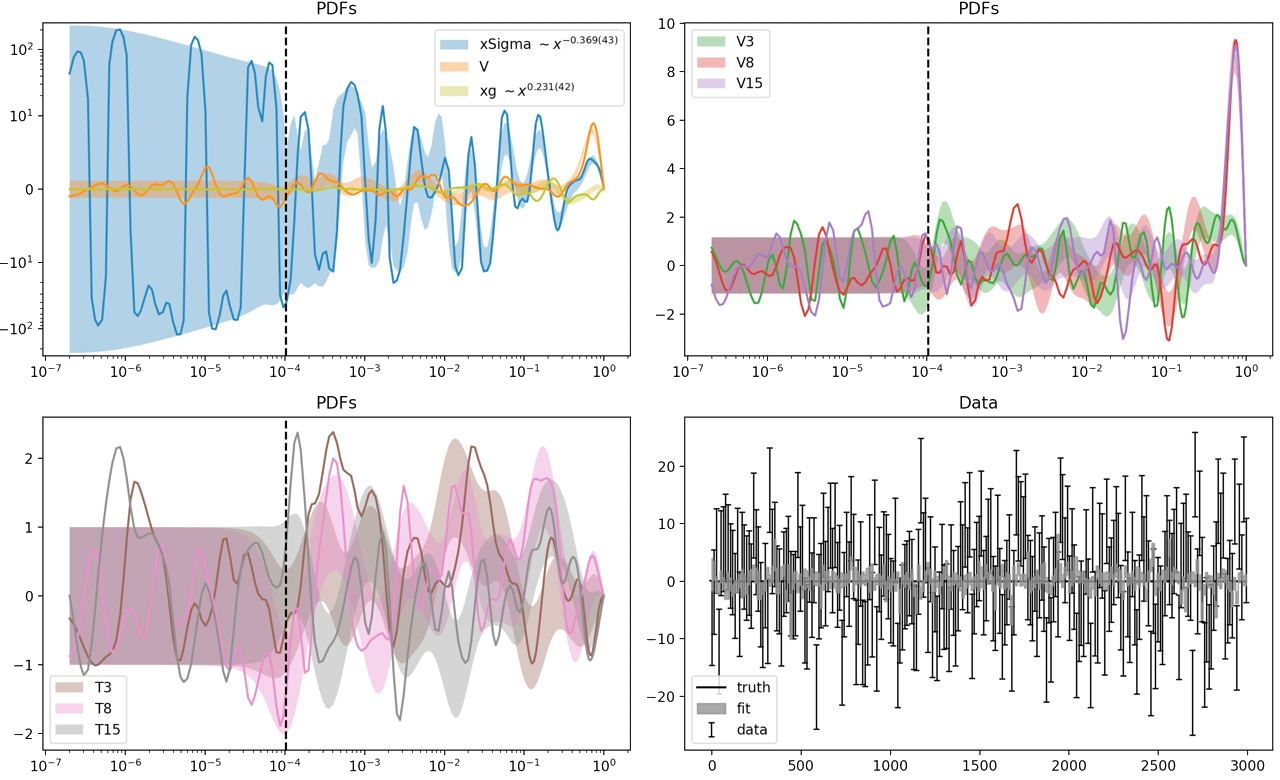
\includegraphics[width=\textwidth]{fit-pdf-new}
                \caption{
                    New fit candidate, with less random data (still pretty
                    random).
                }
            \end{figure} 
        \end{column}
        \begin{column}{0.4\textwidth}
            \begin{figure}
                \centering
                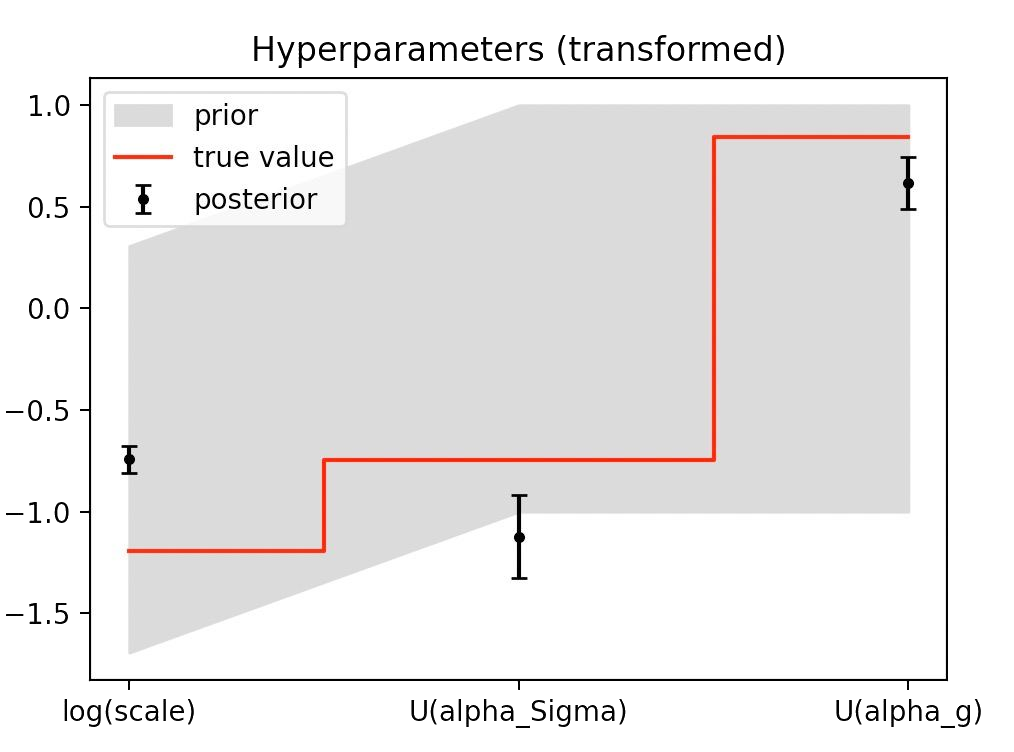
\includegraphics[width=\textwidth]{fit-hyper-new}
                \caption{
                    Hyperparameters fit: notice that while exponents are
                    working, we are still missing the correlation length.
                }
            \end{figure} 
        \end{column}
    \end{columns}
\end{frame}

\end{document}
